\documentclass[aspectratio=169, t, 8pt]{beamer}

%------configurando acentos-----------
\usepackage[utf8]{inputenc}
\usepackage[T1]{fontenc}
\usepackage[brazilian]{babel}
\usepackage{montserrat}
\usefonttheme[onlymath]{serif}
\usepackage{booktabs} % Tabelas elegantes sem linhas verticais
\usepackage{multirow}
\usepackage{array}
\usepackage[most]{tcolorbox}
\usepackage{graphicx}
\usepackage{xcolor}
\usepackage{colortbl}
\usepackage{ulem}
\usepackage{enumitem}

\DeclareMathOperator{\sen}{sen}
\DeclareMathOperator{\coss}{cos}
\DeclareMathOperator{\tg}{tg}
%-------Estilos Beamer---------------
\usetheme{metropolis}
%\usecolortheme{crane}
%\usefonttheme{serif}
\linespread{1.2}

% Personalização de Cores (Exemplo: Minimal Teal)
% Cores Base
\definecolor{BgCanvas}{HTML}{F9F9FB}      % Off-white muito suave
\definecolor{MainText}{HTML}{2B2D42}      % Grafite escuro para alta legibilidade
\definecolor{PrimaryAccent}{HTML}{15407f} % Azul poeira (Dusty Blue)

% Tons Pastéis para Destaques e Cards
\definecolor{PastelGreenBg}{HTML}{E8F0EC}  % Sálvia Claro (Sucesso / Destaque Positivo)
\definecolor{PastelGreenFg}{HTML}{2D5A44}

\definecolor{PastelCoralBg}{HTML}{FDEAE6}  % Coral Soft (Atenção / Problema / Alerta)
\definecolor{PastelCoralFg}{HTML}{7A3025}

\definecolor{PastelPurpleBg}{HTML}{F0EBF4} % Lavanda (Conceitos / Citações)
\definecolor{PastelPurpleFg}{HTML}{4A3E56}

\definecolor{PastelYellowBg}{HTML}{FFF4E6} % Areia / Manteiga (Notas / Dados Secundários)
\definecolor{PastelYellowFg}{HTML}{7A522A}

% --- CONFIGURAÇÕES DE TEMA BEAMER ---
%\usetheme{metropolis}

\setbeamertemplate{itemize item}{\textcolor{MainText}{$\bullet$}}
\setbeamertemplate{itemize subitem}{\textcolor{MainText}{\scriptsize$\circ$}}
\setbeamertemplate{itemize 3rditem}{\textcolor{MainText}{\tiny$\blacksquare$}}

\setbeamercolor{background canvas}{bg=BgCanvas}
\setbeamercolor{normal text}{fg=MainText}
\setbeamercolor{frametitle}{bg=PastelGreenFg, fg=BgCanvas}
\setbeamercolor{title}{fg=MainText}
\setbeamercolor{subtitle}{fg=PrimaryAccent}
\setbeamercolor{structure}{fg=PrimaryAccent}

% Remove a linha amarela padrão do Metropolis sob o título
\setbeamertemplate{title separator}{}
\setbeamertemplate{progress bar in section page}{}

% ==============================================================================
% PALETA DE CORES "AZUL MATEMÁTICO" (Inspirada na imagem)
% ==============================================================================
\definecolor{BgCream}{HTML}{FFFDFB}       % Fundo creme suave
\definecolor{TextDark}{HTML}{1A2530}      % Texto em castanho escuro elegante
\definecolor{PrimaryBlue}{HTML}{0F52BA}  % Laranja vibrante (Títulos e destaques)
\definecolor{DeepBlue}{HTML}{082846}     % Terracota queimado (Alertas)
\definecolor{SoftBlue}{HTML}{E6F0FA}     % Laranja bem suave (Fundo de blocos)

% =================================================
% CONFIGURAÇÃO DO TEMA METROPOLIS
% =================================================
% Cores do texto e fundo geral
\setbeamercolor{normal text}{fg=TextDark, bg=BgCream}
\setbeamercolor{alerted text}{fg=DeepBlue}
\setbeamercolor{example text}{fg=PrimaryBlue}

% Barra de título dos slides (Frametitle)
\setbeamercolor{frametitle}{fg=BgCream, bg=PrimaryBlue}

% Título principal da apresentação (Slide de Capa)
\setbeamercolor{titlelike}{fg=PrimaryBlue}
\setbeamercolor{subtitle}{fg=DeepBlue}

% Barra de progresso (Linha do Metropolis)
\setbeamercolor{progress bar}{fg=PrimaryBlue, bg=PrimaryBlue!20}

% Customização de Blocos (block, alertblock, exampleblock)
\setbeamercolor{block title}{fg=BgCream, bg=PrimaryBlue}
\setbeamercolor{block body}{fg=TextDark, bg=SoftBlue}

\setbeamercolor{block title alerted}{fg=BgCream, bg=DeepBlue}
\setbeamercolor{block body alerted}{fg=TextDark, bg=DeepBlue!15}


% --- ESTILOS DE CARDS PASTEL COM TCOLORBOX ---
\newtcolorbox{cardPrincipal}[1][]{
  colback=SoftBlue,
  colframe=DeepBlue,
  coltext=TextDark,
  arc=6pt,
  boxrule=0pt,
  left=12pt, right=12pt, top=10pt, bottom=10pt,
  fonttitle=\bfseries\small,
  #1
}

\newtcolorbox{cardcoral}[1][]{
  colback=PastelCoralBg,
  colframe=PastelCoralFg,
  coltext=PastelCoralFg,
  arc=6pt,
  boxrule=0pt,
  left=12pt, right=12pt, top=10pt, bottom=10pt,
  fonttitle=\bfseries\small,
  #1
}

\newtcolorbox{cardpurple}[1][]{
  colback=PastelPurpleBg,
  colframe=PastelPurpleFg,
  coltext=PastelPurpleFg,
  arc=6pt,
  boxrule=0pt,
  left=12pt, right=12pt, top=10pt, bottom=10pt,
  fonttitle=\bfseries\small,
  #1
}

\newtcolorbox{cardyellow}[1][]{
  colback=PastelYellowBg,
  colframe=PastelYellowFg,
  coltext=PastelYellowFg,
  arc=6pt,
  boxrule=0pt,
  left=12pt, right=12pt, top=10pt, bottom=10pt,
  fonttitle=\bfseries\small,
  #1
}

\graphicspath{{../../src/img/semana10/}}

%--------Dados do Documento
\title{O Conceito de Função}
\subtitle{}
\author{prof. Eduardo}
\institute{Pré-Universitário Oficina do Saber / UFF}

\date{\today}


%-------- Pacotes Matemática -------------
\usepackage{amsmath}
\usepackage{amsthm}
\usepackage{amsfonts}
\usepackage{amssymb}
\usepackage{xfrac}
\usepackage{thmtools}

\begin{document}

    \begin{frame} %capa
        \vspace*{\fill}
            
            \begin{columns}[c]
                \begin{column}{0.5\textwidth}
                    {\usebeamerfont{title}\usebeamercolor[fg]{title}\inserttitle}\vspace{0.2cm}
                    
                    {\usebeamerfont{subtitle}\usebeamercolor[fg]{subtitle}\insertsubtitle}\vspace{0.5cm}

                {\usebeamerfont{author}\insertauthor}\vspace{0.3cm}

                {\usebeamerfont{institute}\insertinstitute}\vspace{0.3cm}

                {\usebeamerfont{date}\insertdate}
            \end{column}
            
            
            \begin{column}{0.4\textwidth}
                \centering
                
\includegraphics[width=0.4\textwidth]{../logo_ofSaber.png}

                \vspace{.4cm}
                \vspace*{\fill}
        \begin{columns}[c]
            \begin{column}{.5\textwidth}
                \centering
\includegraphics[width=.5\textwidth]{../Proex02c.png}
            \end{column}
            \begin{column}{.5\textwidth}
                \centering
\includegraphics[width=0.4\textwidth]{../Logo_UFF.png}
            \end{column}
        \end{columns}
        \vspace*{\fill}
            \end{column}
        \end{columns}
    \vspace*{\fill}
    \end{frame}

    % \frame
        % {
        %     \usebackgroundtemplate{
        %     \includegraphics[width=\paperwidth]{segunda_capa_pitagoras.png}}
        %     \begin{frame}[plain]                
        %     \end{frame}
        % }

    \begin{frame}{Relações}
        \begin{columns}[totalwidth=.9\textwidth, T]
            \begin{column}{.45\textwidth}
                {\Large                    
                    \[
                        \begin{aligned}
                            &\text{Relação de ordem: } a \leq b\\
                            \vspace{1.2em}
                            &\text{Relação de pertencimento: } a \in A\\
                            \vspace{1.2em}
                            &\text{Relação de igualdade: } a = b\\
                            \vspace{1.2em}
                            &\text{Relação de função:} \; f(x): y=ax^2 +3 
                        \end{aligned}
                    \]
                }
            \end{column}

            \begin{column}{.35\textwidth}
                Dados dois conjuntos $A$ e $B$, definimos uma relação $R$ sobre $A$ e $B$ como uma associação ente elementos $x \in A$ e $y \in B$, mediante uma lei determinada.

                \vspace{1.em}

                O tempo todo fazemos usos de algumas relações, em Matemática, sem que nos demos conta. Ao lado temos alguns exemplos.
            \end{column}
        \end{columns}
    \end{frame}

    \begin{frame}{Funções}
        \begin{columns}[totalwidth=0.9\textwidth]
            \begin{column}{.45\textwidth}
                \begin{figure}
                    \centering
                    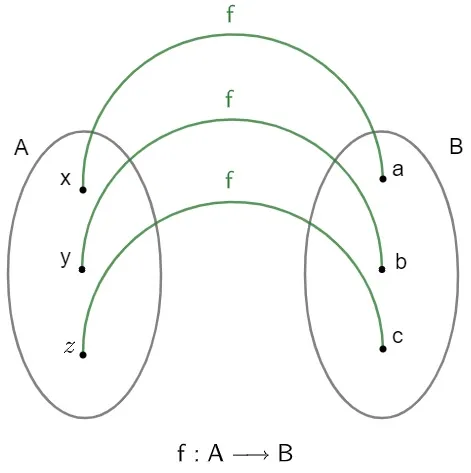
\includegraphics[width=.8\textwidth]{funcoes_definicao.png}
                \end{figure}                
            \end{column}
            \begin{column}{.45\textwidth}
                Uma função é um tipo especial de relação entre dois conjuntos não-vazios. Um deles, chamado Domínio e o outro, chamado Contradomínio.

                Cada elemento do Domínio pode se relacionar com um, e somente um, elemento do Contradomínio. 

                \vspace{1.2em}

               Funções são importantes ferramentas matemáticas para {\it modelarem} fenômenos da natureza, comportamentos da economia, visualização de dados estatísticos, etc.
            \end{column}
        \end{columns}
    \end{frame}

    \begin{frame}{Visualizando Funções - 1}
        \vspace{1.2em}
        \begin{columns}[totalwidth=.9\textwidth]
            \begin{column}{.9\textwidth}
                \centering
                \begin{tabular}{|c|c|c|c|}
                    \hline
                    {\bf Nome} & {\bf Idade} & {\bf Time} & {\bf irmãos}\\
                    \hline
                    Andreia & 23 & Flamengo & Osvaldo\\
                    \hline
                    Reginaldo & 17 & Flamengo & Elaine, Aparecida\\
                    \hline
                    Osvaldo & 32 & Flamengo & Andreia\\
                    \hline
                    Joseane & 17 & Vasco & --- \\
                    \hline
                \end{tabular}

                \vspace{1.2em}

                \begin{figure}
                    \centering
                    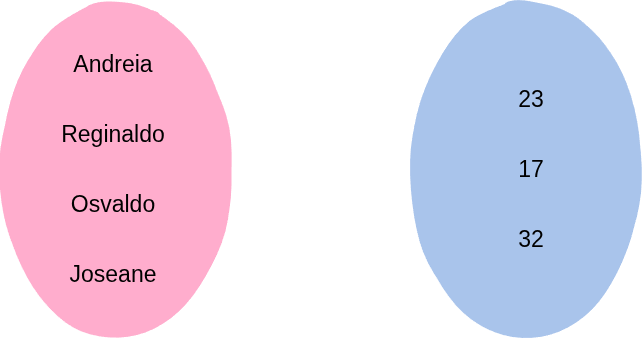
\includegraphics[width=.6\textwidth]{diagrama_01.png}
                \end{figure}
            \end{column}

        \end{columns}
    \end{frame}

    \begin{frame}{Visualizando Funções - 2}
        \vspace{1.2em}
        \begin{columns}[totalwidth=.9\textwidth]
            \begin{column}{.9\textwidth}
                \centering
                \begin{tabular}{|c|c|c|c|}
                    \hline
                    {\bf Nome} & {\bf Idade} & {\bf Time} & {\bf irmãos}\\
                    \hline
                    Andreia & 23 & Flamengo & Osvaldo\\
                    \hline
                    Reginaldo & 17 & Flamengo & Elaine, Aparecida\\
                    \hline
                    Osvaldo & 32 & Flamengo & Andreia\\
                    \hline
                    Joseane & 17 & Vasco & --- \\
                    \hline
                \end{tabular}

                \vspace{1.2em}

                \begin{figure}
                    \centering
                    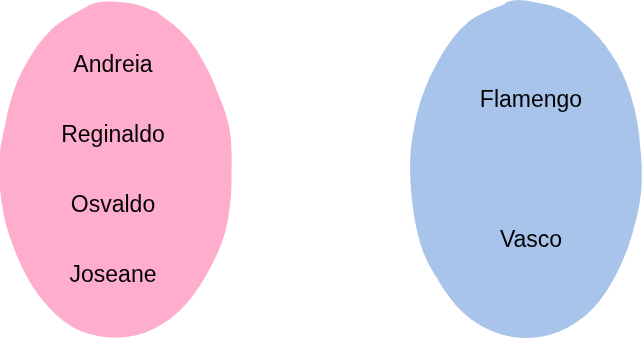
\includegraphics[width=.6\textwidth]{diagrama_02.png}
                \end{figure}
            \end{column}

        \end{columns}
    \end{frame}

    \begin{frame}{Visualizando Funções - 3}
        \vspace{1.2em}
        \begin{columns}[totalwidth=.9\textwidth]
            \begin{column}{.9\textwidth}
                \centering
                \begin{tabular}{|c|c|c|c|}
                    \hline
                    {\bf Nome} & {\bf Idade} & {\bf Time} & {\bf irmãos}\\
                    \hline
                    Andreia & 23 & Flamengo & Osvaldo\\
                    \hline
                    Reginaldo & 17 & Flamengo & Elaine, Aparecida\\
                    \hline
                    Osvaldo & 32 & Flamengo & Andreia\\
                    \hline
                    Joseane & 17 & Vasco & --- \\
                    \hline
                \end{tabular}

                \vspace{1.2em}

                \begin{figure}
                    \centering
                    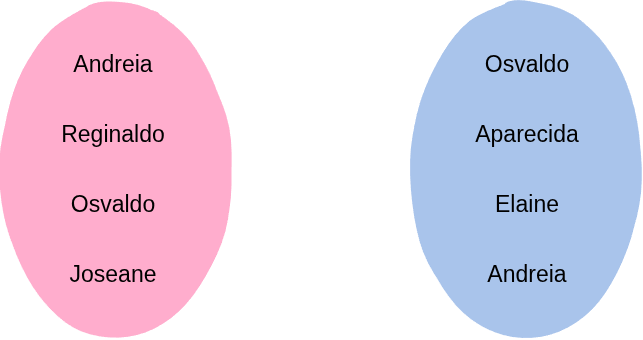
\includegraphics[width=.6\textwidth]{diagrama_03.png}
                \end{figure}
            \end{column}
        \end{columns}

    \end{frame}
    
    \begin{frame}{Funções: Expressão Algébrica}
       \begin{columns}[totalwidth=.9\textwidth]
         \begin{column}{.45\textwidth}
            \large\[
                \begin{aligned}
                    &f(x) = x + 2\\
                    &g(x) = \sen{(x+2)}\\
                    &h(x) = (x+2)^3 \\
                    &k(x) = k^2 + 2k + 4
                \end{aligned}
            \]
        \end{column}
        \begin{column}{.45 \textwidth}
            Então, quando relacionamos os elementos de um conjunto A (domínio) aos elementos de um conjunto B (contradomínio), de modo que tenhamos uma função,podemos dizer que os elementos de B estão em função de A.

            De modo geral escrevemos algebricamente uma função da seguinte forma:

            \vspace{1.2em}

                {\large
                \[
                    f: A \rightarrow B
                \]}

                {\large
                \[
                    y = f(x)
                \]
                }

            Matematicamente $f(x)$ pode ser escrita como uma expressão com $x$ como incógnita.
        \end{column}
       \end{columns}
    \end{frame}

    \begin{frame}{Domínio, Contradomínio e Imagem}
        \begin{columns}[totalwidth=.9\textwidth]
            \begin{column}{.45\textwidth}
                \begin{figure}
                    \centering
                    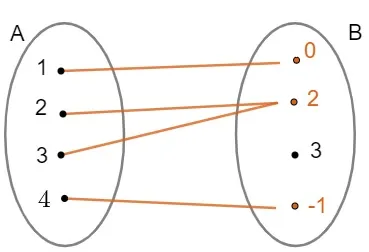
\includegraphics[width=.8\textwidth]{dominio-contradominio.png}
                \end{figure}
            \end{column}
            \begin{column}{.45\textwidth}
                Na relação entre conjuntos domínio e contradomínio, temos um subconjunto especial, chamado {\bf imagem}. Este é o subconjunto do domínio cujos elementos est~ao em função dos elementos do domínio.

                \vspace{1.2em}

                Na imagem ao lado, temos:

                \[
                    \begin{aligned}
                        & D = A = \{1,2,3,4\} \\
                        & CD = B = \{-1,0,2,3\}\\
                        & Im = \{-1,0,2\}
                    \end{aligned}
                \]
            \end{column}
        \end{columns}
    \end{frame}

    \begin{frame}{Domínio, Contradomínio e Imagem}
        \begin{columns}[totalwidth=.9\textwidth]
            \begin{column}{.45\textwidth}
                \Large
                \[
                    f(x) = x^2
                \]

                \vspace{3em}

                \[
                    f(x) = \frac{1}{x-8}
                \]

                \vspace{3em}

                \[
                    f(x) = \sqrt{4-x}
                \]
            \end{column}
            \begin{column}{.45\textwidth}
                No caso de funções definidas por expressões, o domínio será dado pelos valores de $x$ que tornam a expressão verdadeira e o conjunto Imagem é o conjunto dos valores definidos para cada valor dado de $x$.
            \end{column}
        \end{columns}        
    \end{frame}

    \begin{frame}{Tipos de Funções}
        \begin{columns}[totalwidth=.9\textwidth]
            \begin{column}{.45\textwidth}
                \begin{figure}
                    \centering
                    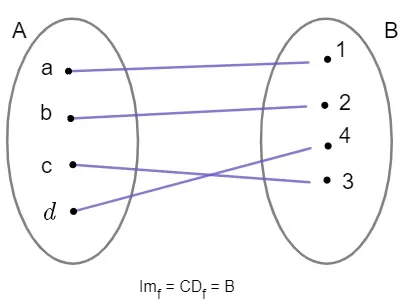
\includegraphics[width=.6\textwidth]{funcao-sobrejetora.jpg}

                    \vspace{1.2em}
                    
                    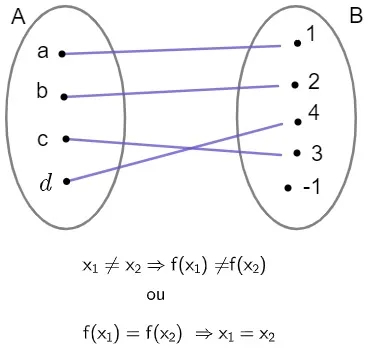
\includegraphics[width=.6\textwidth]{funcao-injetora.jpg}
                \end{figure}
            \end{column}

            \begin{column}{.45\textwidth}
                Podemos classificar as funções em três tipos, de acordo com as relações entre domínio e contradomínio:

                \begin{itemize}
                    \item {\bf Função Sobrejetiva}. É a função em que todo elemento elemento do contradomínio é também elemento da imagem ($CD = Im$).
                    \item {\bf Função Injetiva}. É aquela em que cada elemento da imagem se relaciona a um elemento do domínio. Perceba que não há a necessidade de todo elemento do contradomínio estar relacionado a um elemento do domínio.
                    \item {\bf Função Sobrejetiva} É a função que é sobrejetiva e injetiva ao mesmo tempo.
                \end{itemize}
            \end{column}
        \end{columns}
    \end{frame}

    \begin{frame}{Funções Compostas}
        \begin{columns}[totalwidth=.9\textwidth]
            \begin{column}{\textwidth}
                \begin{figure}
                    \centering
                    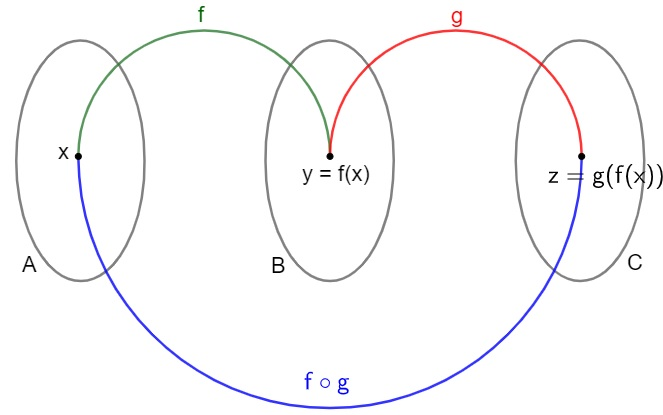
\includegraphics[width=.6\textwidth]{funcao-composta.png}
                \end{figure}

                A composição de funções pode ser entendida como um atalho entre três conjuntos $A,B,C$.Perceba no diagrama acima que o conjunto $B$ é contradomínio de $A$ e domínio do conjunto $B$. A composição de conjuntos escreve o conjunto $C$ como função da função $f(x)$. Isso é como se os elementos de $A$ fossem diretamente relacionados aos elementos de $C$.
            \end{column}
        \end{columns}
    \end{frame}

    \begin{frame}{Exemplo de Função Composta}
        \begin{columns}[totalwidth=.9\textwidth]
            \begin{column}{.45\textwidth}
                
            \end{column}
            \begin{column}{.45\textwidth}
                Imagine que você está comprando um produto em uma loja on-line. Para esta compra, você dispões de um cupom de desconto de 10\% no preço da mercadoria e pagará um custo fixo no frete, de $R\$ \, 15,00$.

                \vspace{1.2em}

                Podemos representar as situações com duas funções:

                \vspace{1.2em}

                1. Preço com desconto: $p(x) = 0,9x$;

                2. Taxa de entrega: $t(y)=y+15$

                \vspace{1.2em}

                Podemos pensar que o valor final com a taxa dependerá do preço da mercadoria com desconto. Portanto ao invés de calcularmos passo a passo, podemos calcular diretamente:

                \vspace{1.2em}

                $t(p(x)) = p(x) + 15 \quad \therefore \quad t(x) = 0,9x + 15$
            \end{column}
        \end{columns}
    \end{frame}

%----------------------------------------------
%              EXERCÍCIOS
%----------------------------------------------

    \begin{frame} {Exercícios} %Gabarito 1-C
        \begin{columns}
            \centering
            \begin{column}{.9\textwidth}
                1. Em uma indústria metalúrgica o custo de produção de uma peça automotiva corresponde a um custo fixo mensal de R\$ 5 000,00 acrescido de um custo variável de R\$ 55,00 por unidade produzida mais 25\% de impostos sobre o custo variável.
                
                Considerando que o preço de venda dessa peça pela indústria aos comerciantes é de R\$ 102,00, determine:

                \vspace{1.2em}

                \begin{itemize}
                    \item {\bf a.)} A função custo da produção de x peças.
                    \item {\bf b.)} A função receita referente a venda de x peças.
                    \item {\bf c.)} A função lucro na venda de x peças.
                    \item {\bf d.)} O lucro obtido com a venda de 500 unidades. 
                \end{itemize}
            \end{column}    
        \end{columns}
    \end{frame}

    \begin{frame} {Exercícios} %Gabarito 2-B
        \begin{columns}[totalwidth=.9\textwidth]
            \begin{column}{\textwidth}
                2. Em uma indústria, o processo de fabricação de um componente eletrônico passa por duas máquinas consecutivas. O tempo de operação (em minutos) da primeira máquina depende da quantidade $x$ de matéria-prima inserida e é modelado pela função $g(x) = x^2 - 2x$. Imediatamente após, a peça passa para a segunda máquina, cujo custo de operação (em reais) em função do tempo $t$ (em minutos) que a peça ficou na primeira máquina é dado por $f(t) = 3t + 15$.
                
                \vspace{1em}

                Se um lote utilizar $4\text{ kg}$ de matéria-prima ($x = 4$), qual será o custo de operação na segunda máquina?

                \begin{enumerate}[label=\alph*)]
                    \item $R\$ \, 15,00$
                    \item $R\$ \, 24,00$
                    \item $R\$ \, 39,00$
                    \item $R\$ \, 45,00$
                    \item $R\$ \, 51,00$
                \end{enumerate}
            \end{column}
        \end{columns}
    \end{frame}

    \begin{frame}{Exercícios}
        \begin{columns}[totalwidth=.9\textwidth]
           \begin{column}{\textwidth}
            3. Uma escola organiza uma gincana de matemática e define uma função $f: A \rightarrow B$, onde o conjunto $A$ (Domínio) é formado pelos 40 alunos de uma turma, e o conjunto $B$ (Contradomínio) é formado pelas 4 equipes da gincana: {Alfa, Beta, Gama, Delta}. A regra de associação dessa função determina que cada aluno (elemento de $A$) seja mapeado para a equipe (elemento de $B$) na qual foi sorteado para competir.
            
            \vspace{1em}

            Para que a função construída por esse sorteio seja rigorosamente classificada como sobrejetora, qual das situações abaixo deve obrigatoriamente ocorrer?

            \vspace{1.2em}

                \begin{enumerate}[label=\alph*)]
                    \item Cada equipe deve receber exatamente 10 alunos, garantindo uma divisão igualitária.
                    \item Nenhum aluno da turma pode ficar sem ser sorteado para uma equipe.
                    \item Nenhuma das quatro equipes pode terminar o sorteio sem receber pelo menos um aluno.
                    \item Cada aluno deve poder escolher em qual equipe deseja participar.
                    \item Dois alunos não podem ser sorteados para a mesma equipe.
                \end{enumerate}
           \end{column}
        \end{columns}        
    \end{frame}

    \begin{frame}{Exercícios}
        \begin{columns}[totalwidth=.9\textwidth]
            \begin{column}{\textwidth}
                Uma empresa de aluguel de patinetes elétricos cobra de seus usuários uma taxa fixa de desbloqueio do equipamento no valor de R\$ 3,00, acrescida de R\$ 0,50 por minuto de uso. Para incentivar o uso prolongado, a empresa lançou uma promoção: em viagens que ultrapassem 30 minutos, o usuário recebe um desconto de 20\% sobre o valor total final da corrida.
                
                \vspace{1.2em}

                A expressão algébrica que modela o custo final $C(x)$, em reais, para um usuário que aluga o patinete por $x$ minutos, sabendo que ele andou por mais de meia hora ($x > 30$), é dada por:

                \vspace{1.2em}

                \begin{enumerate}[label=\alph*)]
                    \item $C(x)=2,40+0,40x$
                    \item $C(x) = 3,00 + 0,40x$
                    \item $C(x) = 2,40 + 0,50x$
                    \item $C(x) = 3,00 + 0,50x - 0,20$
                    \item $C(x) = 0,80 \cdot (0,50x)$
                \end{enumerate}
            \end{column}
        \end{columns}
    \end{frame}

\end{document}